\documentclass{webofc}
\usepackage[varg]{txfonts}   % Web of Conferences font

\usepackage{float}
\usepackage[caption = false]{subfig}
%\usepackage[final]{graphicx}

\begin{document}

\title{Trident : An Automated System Tool for \\Collecting and Analyzing Hardware Performance Counters}

\author{\firstname{Servesh} \lastname{Muralidharan}\inst{1}\fnsep\thanks{\email{servesh.muralidharan@cern.ch}} \and
        \firstname{David} \lastname{Smith}\inst{1}\fnsep\thanks{\email{david.smith@cern.ch}}
}

\institute{CERN}

\abstract{%
Trident, a tool to use low level metrics derived from hardware counters to understand Core, Memory and I/O utilisation and bottlenecks. The collection of time series of these low level counters does not induce significant overhead to the execution of the application.

The Understanding Performance team is investigation on a new node characterization tool, `Trident', that can look at various low level metrics with respect to the Core, Memory and I/O. Trident uses a three pronged approach to analysing node's utilisation and understand the stress on different parts of the node based on the given job. Currently core metrics such as memory bandwidth, core utilization, active processor cycles, etc., are being collected. Interpretation of the data is often non intuitive. The tool converts the data into derived metrics that are then represented as a system wide top-down analysis that helps developers and site managers understand the application behavior without the need for in-depth expertise of architecture details.
}
%
\maketitle
%
\section{Motivation}
\label{sec:moti}

Application performance can be characterized by a myriad of tools and techniques. Some of these tools rely on hardware and software performance counters built into a given system to analyze performance bottlenecks. These counters can come from performance monitoring units (PMUs) built into modern processors, storage devices, etc., or from software counters present in the underlying operating system. There is a vast variety of these counters and its often difficult to determine which counters are associated with a particular performance bottleneck in a fast and effective manner. To cater to this an approach called as Top-Down Analysis~\cite{6844459} was proposed, which utilized a hierarchical identification of areas of a processor and its associated metrics that can represent inefficiencies that arise due to this from an application.

The effectiveness of Top-Down analysis lies in the fast identification of performance bottlenecks that arises from the interaction of the application code and the given architecture. However this still relies on classical profiling approach where hotspots are identified in a finite code space that account for a large percentage of the execution time. However typical High-Energy Physics (HEP) code base exhibit sparse compute code spread over several thousand C++ classes. In such a scenario it becomes difficult to use the classical or fine grained profiling approach. In this paper we propose Trident, a tailored profiling tool for such use cases. 

Trident is a coarse grained profiling tool that can quickly identify performance bottlenecks during the runtime of an application by monitoring hardware and software counters. It uses a three pronged approach to simultaneously identify bottlenecks that arise from core, memory or IO subsystem of a given node. The data collection is done in such a way that it causes little to no overhead to the execution of the application. Finally it presents these counters as derived metrics by extending Top-Down analysis and presenting them in a timeline.


\section{Introduction}
\label{sec:intro}

A key requirement for our Trident tool is the ability to collect hardware and software counters with little to no overhead. At the same time we also wanted to support systems with little to no software configuration changes and without the need for elevated privileges for the hardware counter data collection. Due to this we were limited to only few likely options. The easiest and simplest way to record hardware counters appeared to be piggy backing on the \textbf{perf} subsystem[] of the Linux kernel. After setting up a few simple kernel configuration, it was possible for us to record counter data from userspace. While \textbf{perf} supports high level counter names, we found this to drastically vary between kernel versions and architectures. In addition some of the high level counters that we relied do not appear to be directly supported. So therefore we developed a simple architecture identification mechanism using libpfm [] and configured a dynamic set even counters that we validated and tested on a given architecture.

%\begin{figure}
%	\centering
%	\subfloat[fig 1]{\includegraphics[width=0.48\linewidth]{{cmd2.pmpe16.Trident.1.io}.png}}\hfill
%	\subfloat[fig 2]{\includegraphics[width=0.48\linewidth]{{cmd2.pmpe16.Trident.1.me}.png}}\\
%	\subfloat[fig 3]{\includegraphics[width=0.48\linewidth]{{cmd2.pmpe16.Trident.1.cb}.png}}\hfill
%	\subfloat[fig 4]{\includegraphics[width=0.48\linewidth]{{cmd2.pmpe16.Trident.1.co}.png}} 
%\caption{plots of....}
%\label{fig:fig}
%\end{figure}

\section{Design}

\begin{figure}
  \centering
  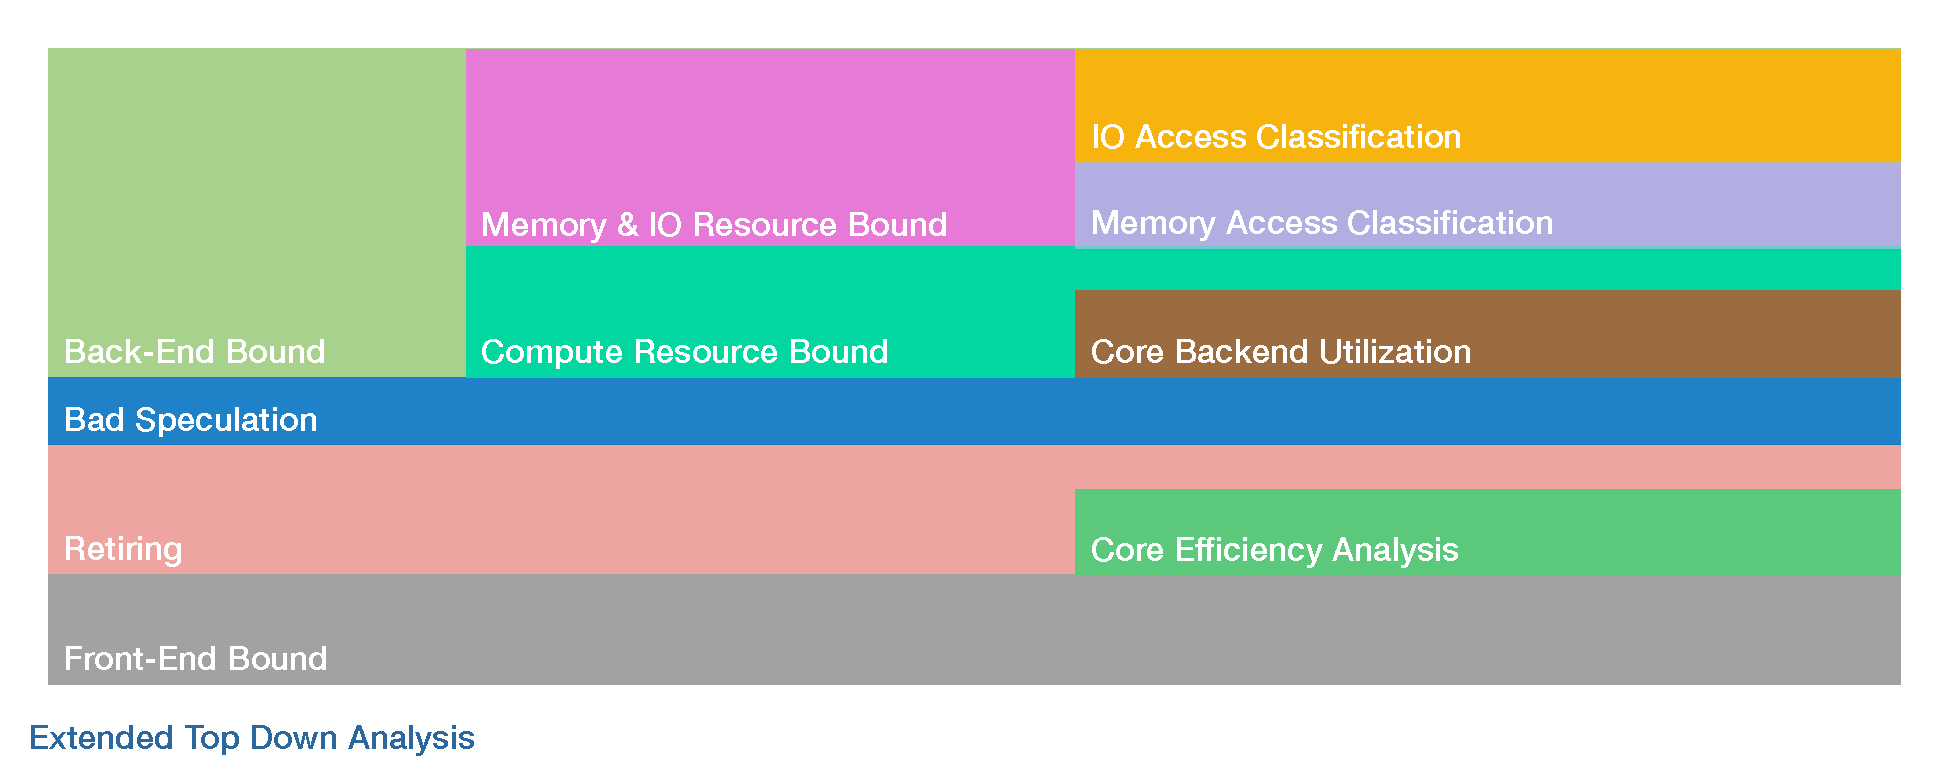
\includegraphics[width=1\linewidth]{ExtendedTopDownDiag.pdf}
\caption{plots of....}
\label{fig:ext_top_down}
\end{figure}

\section{Results}

\begin{figure}
	\centering
	\includegraphics[width=0.8\linewidth]{{cmd2.pmpe16.Trident.1.co}.png}
\caption{plots of....}
\label{fig:at_cmd2_co}
\end{figure}

\begin{figure}
	\centering
	\includegraphics[width=0.8\linewidth]{{cmd2.pmpe16.Trident.1.cb}.png}
\caption{plots of....}
\label{fig:at_cmd2_cb}
\end{figure}

\begin{figure}
	\centering
	\includegraphics[width=0.8\linewidth]{{cmd2.pmpe16.Trident.1.me}.png}
\caption{plots of....}
\label{fig:at_cmd2_me}
\end{figure}

\begin{figure}
	\centering
	\includegraphics[width=0.8\linewidth]{{cmd2.pmpe16.Trident.1.io}.png}
\caption{plots of....}
\label{fig:at_cmd2_io}
\end{figure}

\section{Conclusion}

%For tables use syntax in table~\ref{tab-1}.
%\begin{table}
%\centering
%\caption{Please write your table caption here}
%\label{tab-1}       % Give a unique label
%% For LaTeX tables you can use
%\begin{tabular}{lll}
%\hline
%first & second & third  \\\hline
%number & number & number \\
%number & number & number \\\hline
%\end{tabular}
%% Or use
%\vspace*{5cm}  % with the correct table height
%\end{table}
%
\bibliography{chep18}

\end{document}
